\documentclass[10pt]{article}
\usepackage[polish]{babel}
\usepackage[utf8]{inputenc}
\usepackage[T1]{fontenc}
\usepackage{amsmath}
\usepackage{amsfonts}
\usepackage{amssymb}
\usepackage[version=4]{mhchem}
\usepackage{stmaryrd}
\usepackage{graphicx}
\usepackage[export]{adjustbox}
\graphicspath{ {./images/} }

\begin{document}
\begin{enumerate}
  \item \(W\) trójkącie \(A B C\) na boku \(A B\) dany jest taki punkt \(P\), że \(|A P|:|P B|=2: 5\), a na boku AC taki punkt \(Q\), że \(|A Q|:|Q C|=1: 3\). Proste CP i BQ przecinają się w punkcie S. Prosta AS przecina bok BC w punkcie R. Policz w jakim stosunku punkt R dzieli bok BC.\\
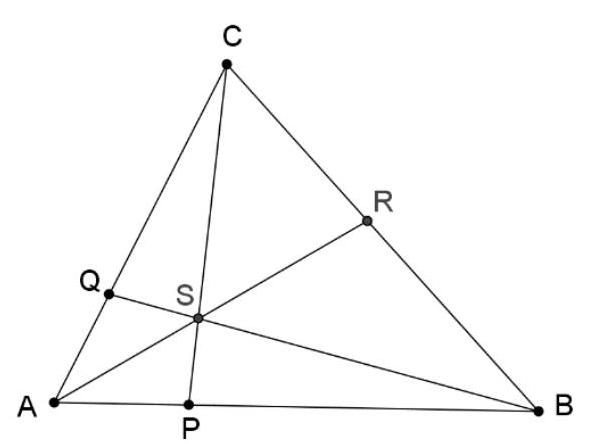
\includegraphics[max width=\textwidth, center]{2024_11_21_bfc1683a10266ed24de7g-1}
  \item Rozważmy następującą grę. Na stole leży 100 cukierków. Gracze na przemian zabierają cukierki ze stołu, nie można jednak wziąć więcej niż 4 (ani mniej niż 1). Wygrywa gracz, który zabierze ostatniego cukierka. Który z graczy ma strategię wygrywającą i jak ona wygląda?
  \item Znajdź wszystkie pary liczb całkowitych ( \(m, n\) ) spełniających równanie:
\end{enumerate}

\[
2 \cdot 3^{n}=7 m+5
\]


\end{document}